% 4
\section{研究概要}



% 4.1
\subsection{概要}
ハンドジェスチャーを使用する際に用いられるセンサーとして、一般的とされているWebカメラではなく、レーザー光を用いる。このことは、従来ジェスチャーを使用できなかったシチュエーションや場所においても、使用することを可能とする。

具体的なレーザー光の使用方法を説明する。多数のレーザーと、それと同数の受光器を用意して、お互いが対面するように配置することにより、その間を手が遮った際に検出できるようにする。この検出した情報から手のおおよその形状を認識する。予め3Dオブジェクトを配置した、三次元の仮想空間を用意して、そこに取得した手の形状を描画し、3Dオブジェクトを動かすことができるようにする。このことで、レーザー光を用いたデバイスがインターフェースとして使用することができることを証明する。

本研究では、これを2台のWebカメラを用いて作ったシミュレータデバイスを用意して実験を行う。



% 4.2
\subsection{提案手法}
\subsubsection{レーザー光デバイス}
レーザー光を用いたハンドジェスチャーを可能とするため、図3-1のようなデバイスを作成した。

\begin{center}
  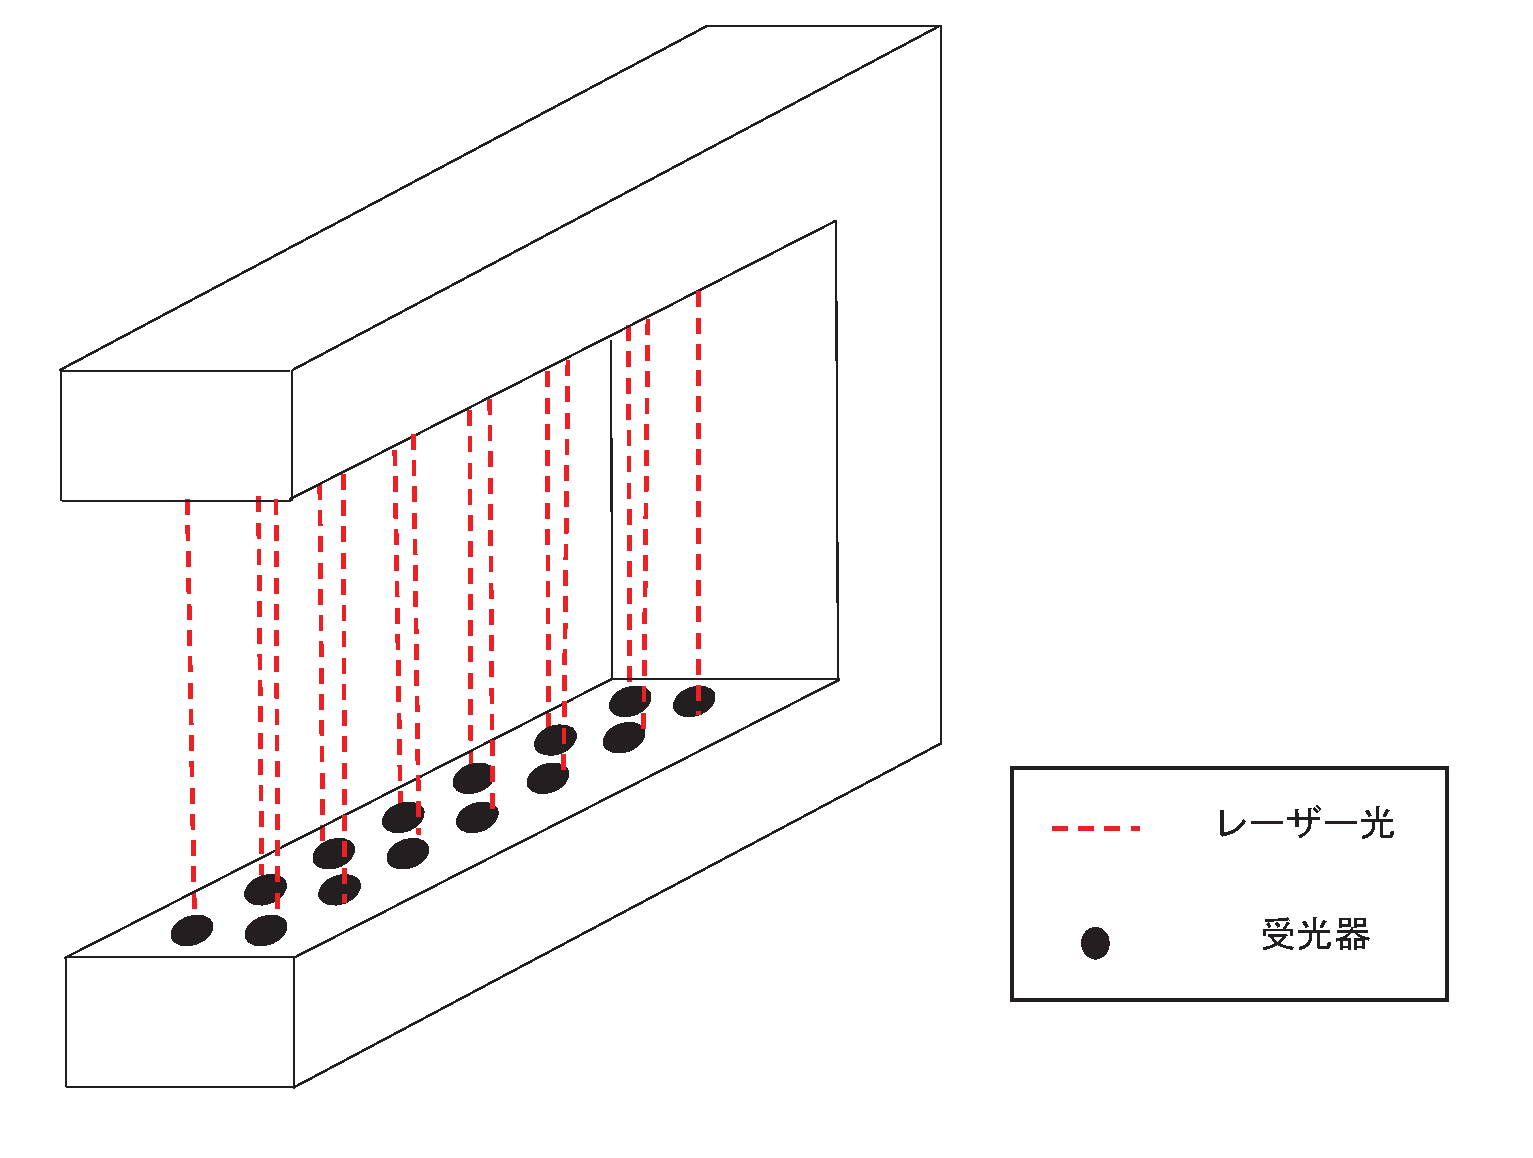
\includegraphics[width=10cm]{RazerDevice_image} \\

 \vspace{1mm}
  図3-1. レーザー光を用いたデバイスのイメージ
\end{center}

デバイスの上部に、計24個のレーザーを設置する。それと対になるように、下部に同数の受光器を設置する。この間を手が通過すると、レーザー光が遮られたことを受光器が検出する。実際に作成したデバイスを用いて、取得した手情報を画像に描画したものを、図3-2に示す。図3-3は使用したデバイスの写真である。

\begin{center}
  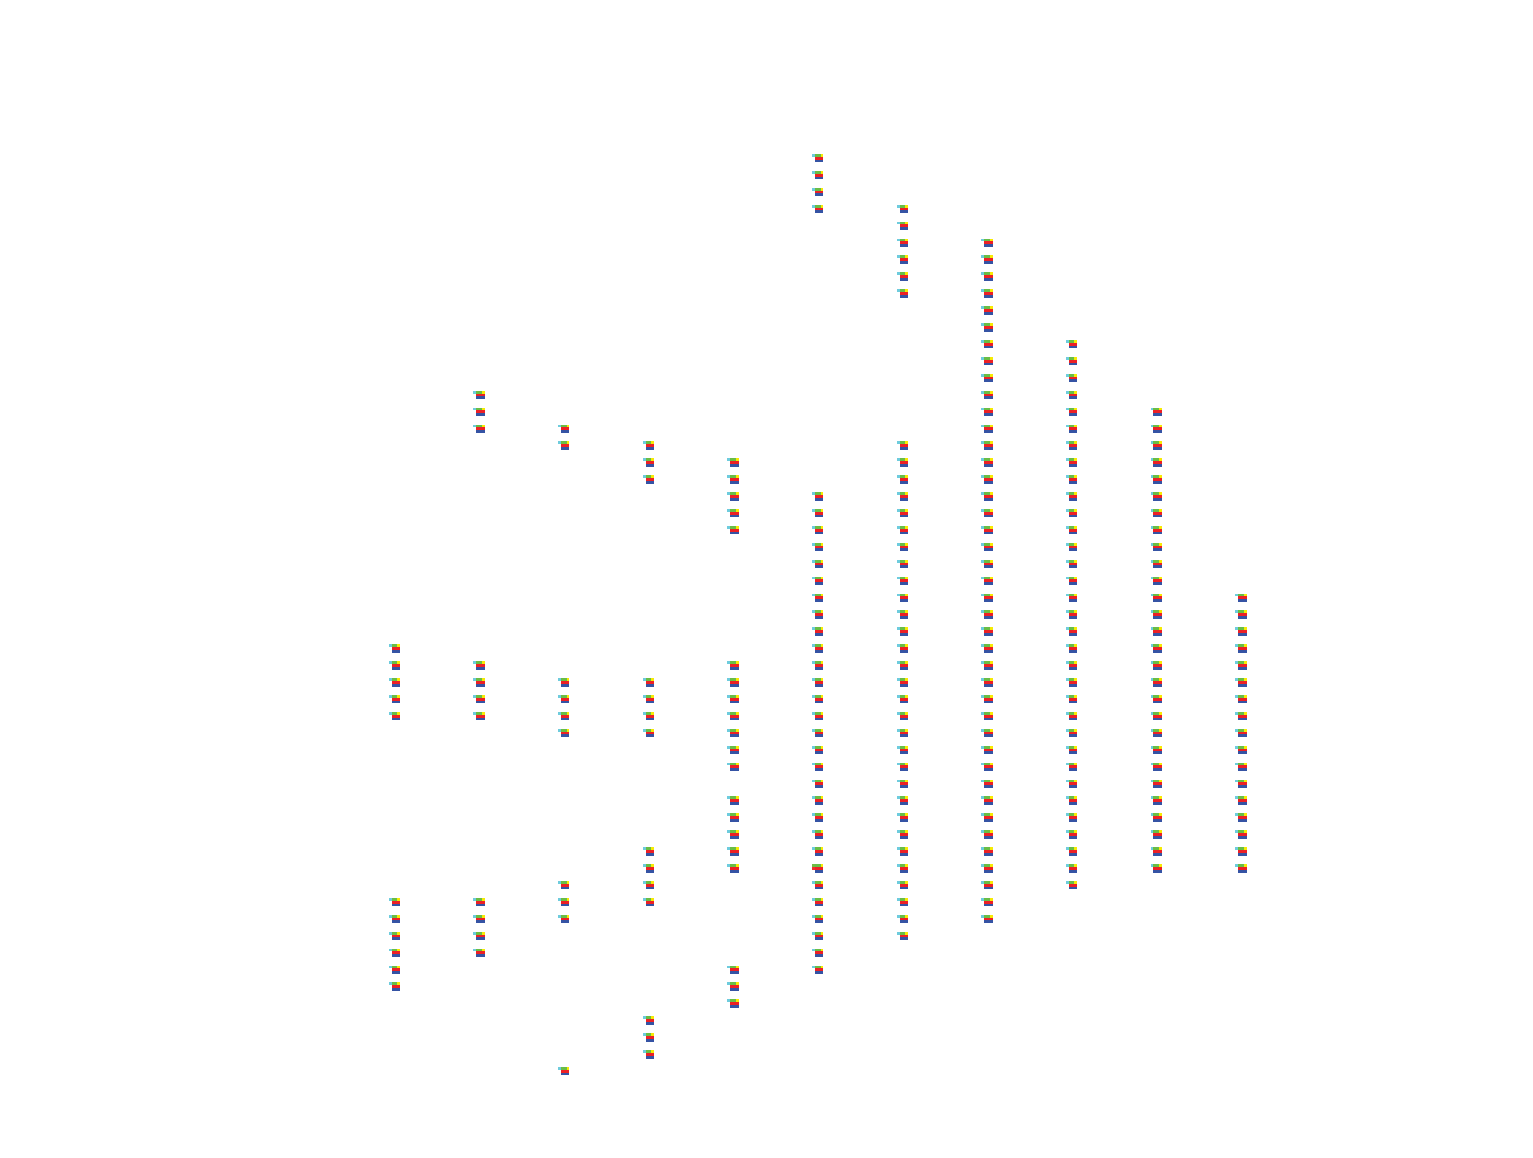
\includegraphics[width=10cm]{RazerDevice_getInfo.eps} \\

 \vspace{1mm}
  図3-2. レーザー光デバイスを用いて実際に得た情報
\end{center}

 \vspace{5mm}

\begin{center}
  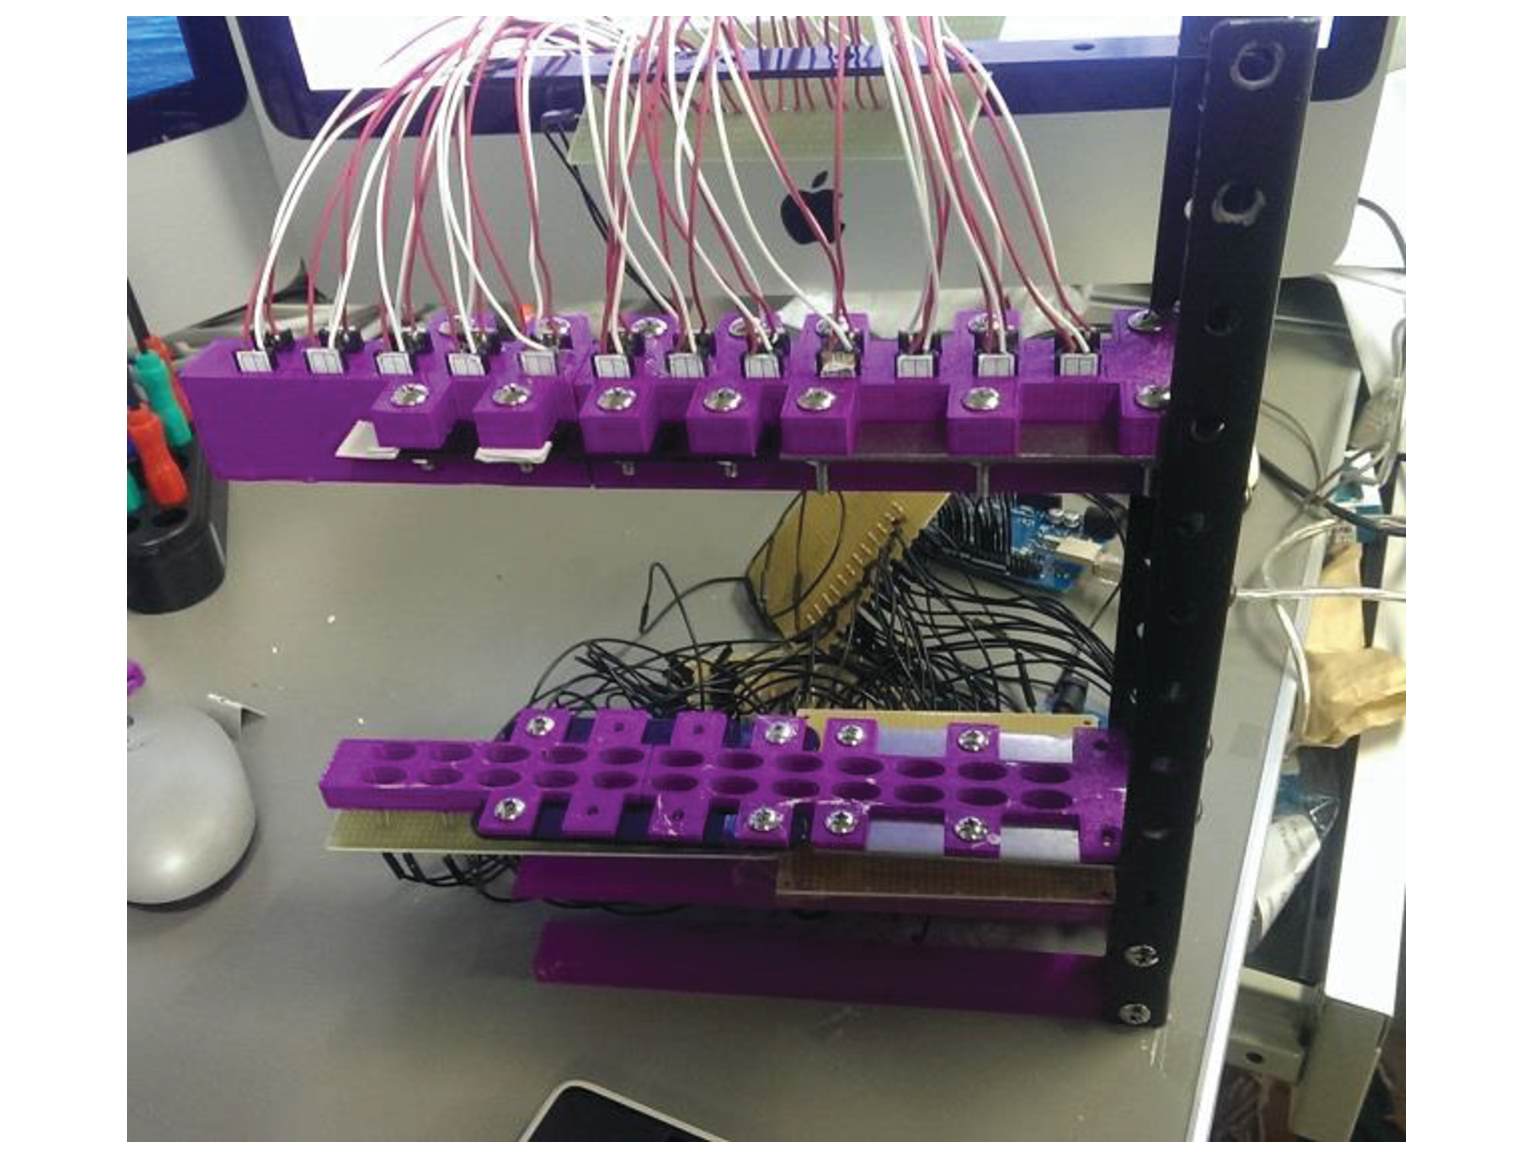
\includegraphics[width=10cm]{RazerDevice_real_color.eps} \\

 \vspace{1mm}
  図3-3. 実際に作成したレーザー光デバイス
\end{center}

図3-2より、レーザー光を用いて手の形状を認識することが可能であることが伺える。しかしながら、このデバイスには問題が存在する。それは、レーザー数が足りないということである。手の情報を得るためには、スキャナーのように手を固定した形で通過させる必要がある。このことは動的な手情報を得ることができないことを示している。つまり、VRと組み合わせた直感的なハンドジェスチャーインターフェースを作ることは、不可能である。だが、図3-2の結果から、手の範囲より広くレーザーを設置することが出来れば、動的に手情報を得ることができると推測される。% このデバイスのイメージ用意してもいいかも
このことを踏まえて、レーザー光の代わりにWebカメラを用いたシミュレータデバイスを作成した。

\subsubsection{Webカメラを用いたシミュレータデバイス}
図3-4は、レーザー光の代わりにWebカメラを用いたシミュレータデバイスのイメージとなる。側面が一つ空いているボックスの上面と側面に対して、図3-4のようにWebカメラを設置する。レーザー光による検出を再現するために、Webカメラから得られた映像に対して、一定間隔毎に情報を取得する座標を設ける。カメラの対面には、青いスクリーンを貼り付けることにより、間を青以外の物体が遮った時、それを検出できるようにする。実際にボックスの中に手を入れて、取得した情報を図3-5に示す。図3-5は図3-4の上部に設置したWebカメラから取得した情報である。同様の手法で、横のWebカメラからも同時に情報を取得する。縦、横の二つの画像から手情報を三次元空間に構築して、同空間に生成したオブジェクトを動かすことにより、直感的なジェスチャーを可能にするための道筋を示す。図3-6は実際に作成したシミュレータデバイスである。

\begin{center}
  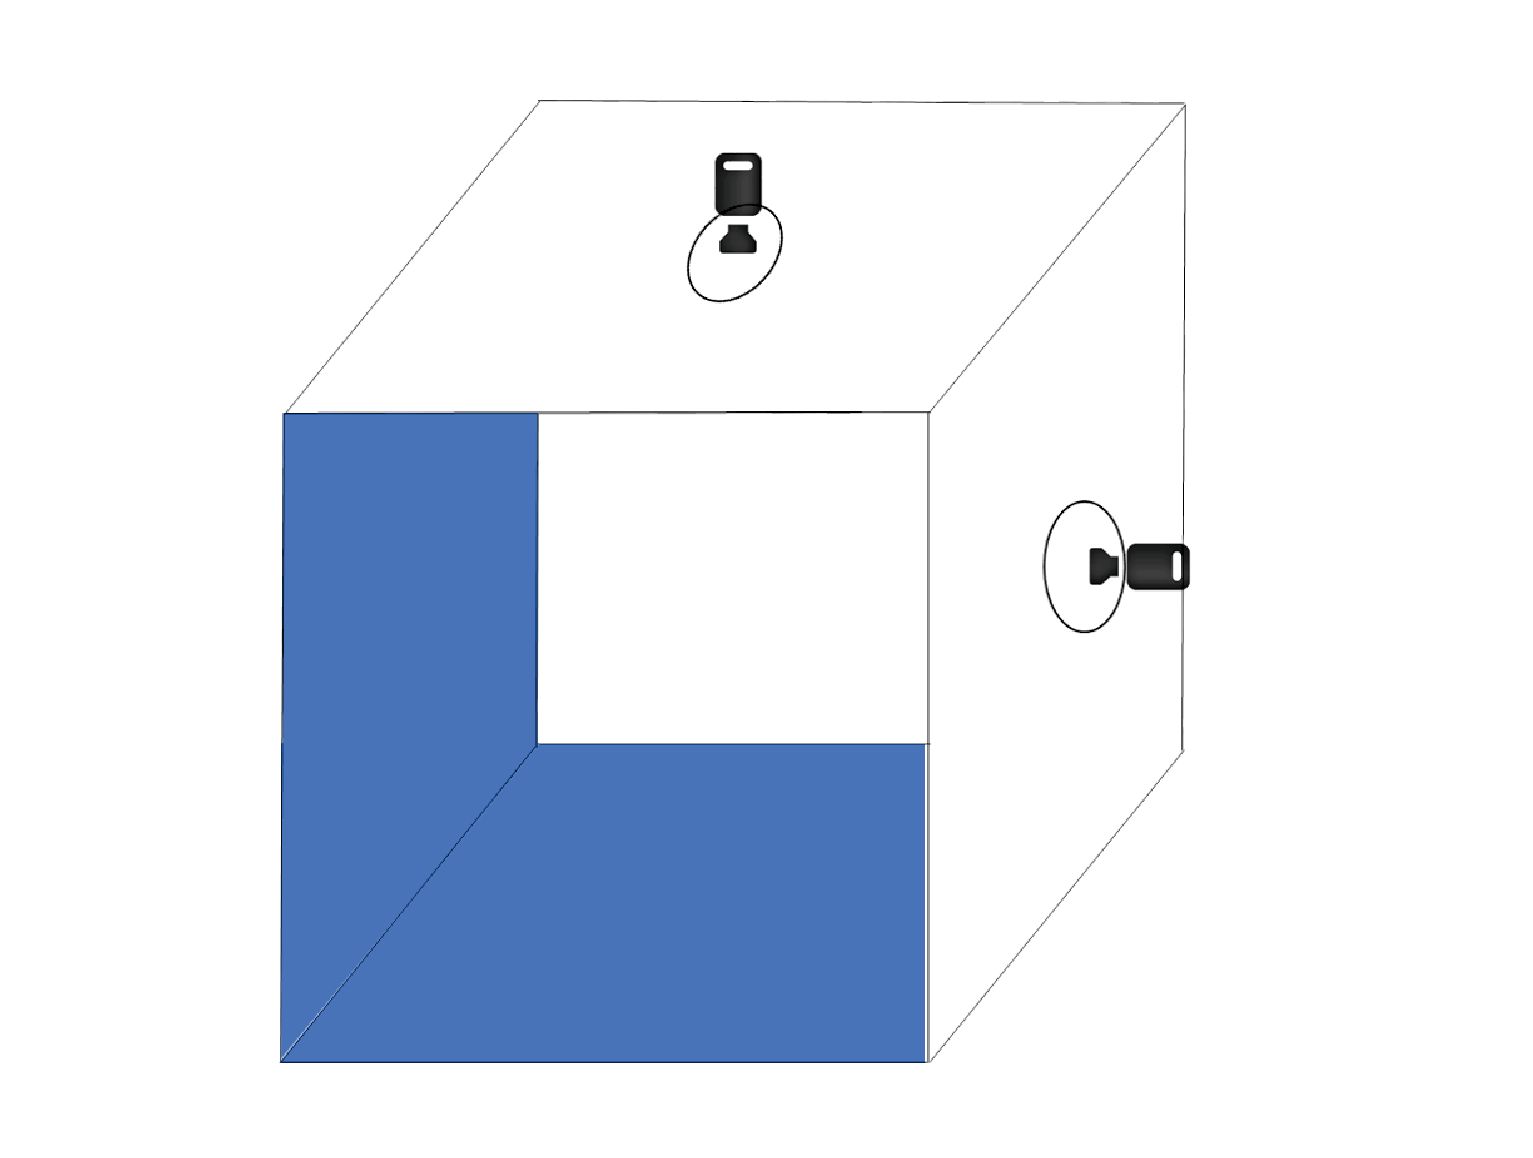
\includegraphics[width=10cm]{Simulator_image.eps} \\

 \vspace{1mm}
  図3-4. Webカメラを用いたシミュレータデバイスのイメージ
\end{center}

\begin{center}
  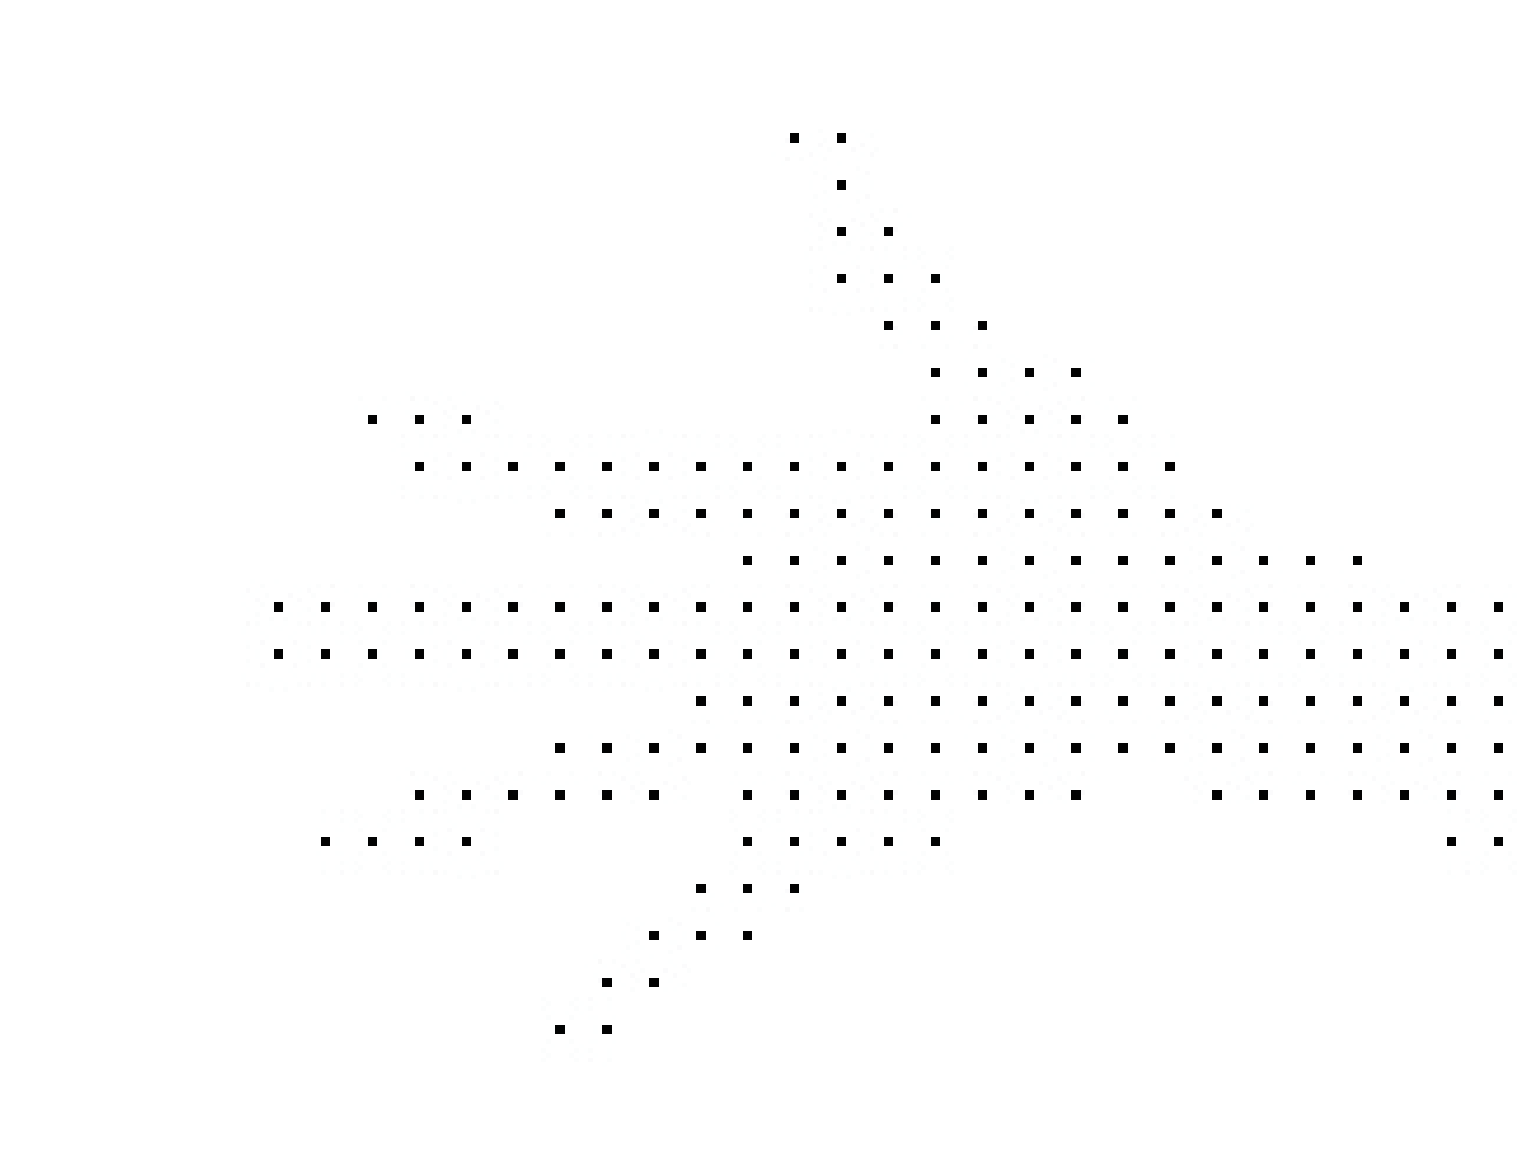
\includegraphics[width=10cm]{Simulator_getInfo.eps} \\

 \vspace{1mm}
  図3-5. シミュレータデバイスから得られた情報
\end{center}

 \vspace{10mm}
\begin{center}
  \includegraphics[width=10cm]{Simulator_real_color.eps} \\

 \vspace{1mm}
  図3-5. 実際に作成したシミュレータデバイス
\end{center}